% Author: Max Melching, 2025
% Lots of styling inspiration from: https://tikz.net/relativity_minkowski_diagram/
\documentclass[border=3pt,tikz]{standalone}

\usepackage{newtxmath}  % Use Times in math mode
\usepackage{tgpagella}  % Use Pagella in text
\usepackage{tikz}
\usepackage{fp}
\usepackage{calc}
\usepackage{pgfkeys}
\usepackage{ifthen}
\usepackage{xcolor}
\usepackage[outline]{contour} % glow around text


\usetikzlibrary{math,arrows.meta,calc,intersections,through,backgrounds,decorations.markings,decorations.pathmorphing}


% -- Styling
\colorlet{lightyellow}{black!10!yellow}
\colorlet{mydarkred}{red!55!black}
\colorlet{myred}{red!85!black}
\colorlet{mydarkorange}{orange!40!yellow!85!black}
\colorlet{mydarkblue}{blue!50!black}


\tikzset{
    >={Stealth[inset=0,angle'=27]},
    light/.style={
        ->,
        lightyellow,
        % line width=0.6,
        semithick,
        decorate,
        decoration={
            snake,
            amplitude=0.5,
            segment length=4.2,
            post length=4.2,
        }
    },
    worldline/.style={
        ->,
        thick,
        black,
    },
    labelledpoint/.style={
        % mydarkred,
        myred,
    },
    simultline/.style={
        mydarkblue,
        dashed,
        % line width=0.4,
        thin,
    }
}


% -- Not styling, this is to Lorentz-transform objects
\tikzset{
    vlorentz/.style={
      cm={1/((1-((#1)*(#1)))^.5,#1*1/((1-((#1)*(#1)))^.5,#1*1/((1-((#1)*(#1)))^.5,1/((1-((#1)*(#1)))^.5,(0,0)}
    },
}



\begin{document}

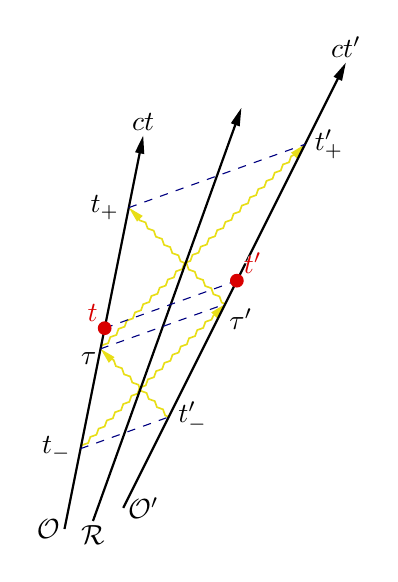
\begin{tikzpicture}

    % -- Set these values to your liking
    % \def\vone{-0.1}
    % \def\vtwo{0.5}
    % \def\tsignal{1}
    % \def\initsep{0}
    % % \def\initsep{1}
    % -- Not working with non-zero \initsep
    % -- -> because clocks are already desynchronized at beginning then...
    % -- -> workaround: choose initsep=0, but start from a later time
    
    % \def\tmin{0}
    % \def\tmax{4.2}


    \def\vone{0.2}
    \def\vtwo{0.5}
    \def\tsignalone{3}
    \def\tsignaltwo{\tsignalone}
    % -- tsignaltwo must be equal to tsignalone for synchrony; change if you want to show how desynchronized observers look like
    % \def\tsignaltwo{2.5}
    \def\initsep{0}

    \def\tmin{2}
    \def\tmax{6.9}
    

    % % \def\vone{0}
    % % \def\vtwo{0}
    % \def\vone{0.2}
    % \def\vtwo{0.2}
    % \def\tsignal{0.5}
    % \def\initsep{1.5}

    % \def\tmin{0}
    % \def\tmax{4.2}


    % \clip (0, 2.8) rectangle (4, 8);  % If you don't like how long certain lines extend

    
    % -- From here on automatic (except you wish to change styling) -----------
    \FPeval{\dopplerone}{((1+\vone)/(1-\vone))^.5}
    \FPeval{\dopplertwo}{((1+\vtwo)/(1-\vtwo))^.5}
    \FPeval{\doppleronetwo}{\dopplertwo/\dopplerone}

    
    \FPeval{\vrelative}{(\vtwo-\vone)/(1-\vone*\vtwo)}
    
    \FPifzero{\vrelative}
        % -- Only initsep is present, just set sensible values
        \FPeval{\vrelativehalf}{0}
        \FPeval{\vreferee}{\vone}
    \else
        \FPeval{\vrelativehalf}{(1-(1-\vrelative*\vrelative)^.5)/\vrelative}
        \FPeval{\vreferee}{(\vone+\vrelativehalf)/(1+\vone*\vrelativehalf)}
    \fi
    

    % -- Calculate relevant coordinates
    \begin{scope}[vlorentz=\vone]
        \coordinate (A) at (0, \tsignalone);
        \coordinate (E) at (0, \doppleronetwo*\tsignaltwo + \initsep);
        \coordinate (B) at (0, \doppleronetwo*\doppleronetwo*\tsignalone + 2*\initsep);
        \coordinate (ABhalf) at ($ (A)!0.5!(B) $);
    \end{scope}

    \begin{scope}[vlorentz=\vtwo]
        \coordinate (C) at (\initsep, \tsignaltwo);
        \coordinate (F) at (\initsep, \doppleronetwo*\tsignalone + \initsep);
        \coordinate (D) at (\initsep, \doppleronetwo*\doppleronetwo*\tsignaltwo + 2*\initsep);
        \coordinate (CDhalf) at ($ (C)!0.5!(D) $);
    \end{scope}
    
    
    % -- Light signals. Separate paths instead of A-F-B for styling reasons
    \draw[light] (A) -- (F);
    \draw[light] (F) -- (B);
    
    \draw[light] (C) -- (E);
    \draw[light] (E) -- (D);

    
    % -- Observer worldlines
    \begin{scope}[
        worldline,
    ]
        \draw[vlorentz=\vone] (0, \tmin) node[left=-2] {$\mathcal{O}$} -- (0, \tmax) node[above=-2] {\contour{white}{$ct$}};

        \draw[vlorentz=\vtwo] (\initsep, \tmin) node[right=-2] {$\mathcal{O}'$} -- (\initsep, \tmax) node[above=-2] {\contour{white}{$ct'$}};

        \draw[vlorentz=\vreferee] ({\initsep/2}, \tmin) node[below=-2] {\contour{white}{$\mathcal{R}$}} -- ({\initsep/2}, \tmax);
    \end{scope}
    

    % -- Lines of Simultaneity
    \begin{scope}[
        simultline,
    ]
        \draw (A) -- (C);
        \draw (B) -- (D);
        \draw (E) -- (F);
        \draw (ABhalf) -- (CDhalf);
    \end{scope}


    % -- Point halfway between emission and reception (= \tau = \tau' if no relative velocity between O, O')
	\draw[fill, labelledpoint] (ABhalf) circle(0.08);
	\draw[fill, labelledpoint] (CDhalf) circle(0.08);


    % -- Labels. Comment if you do not like
    \node[left] at (A) {\contour{white}{$t_-$}};
    \node[right] at (C) {\contour{white}{$t'_-$}};

    \node[left] at (B) {\contour{white}{$t_+$}};
    \node[right] at (D) {\contour{white}{$t'_+$}};

    \node[above left=-1, labelledpoint] at (ABhalf) {\contour{white}{$t$}};
    \node[above right=-1, labelledpoint] at (CDhalf) {\contour{white}{$t'$}};

    \node[below left=-2] at (E) {\contour{white}{$\tau$}};
    \node[below right=-2] at (F) {\contour{white}{$\tau'$}};
\end{tikzpicture}



\end{document}